\chapter{Gomulscy z Anieliny, Wólki Mińskiej, Mikanowa i~Karoliny}

% Przednia okładka podrozdziału
\includepdf{Anielina_mapa_fin.png}

\section{Anielina: 1853~r. - 2025~r.}

Wieś Anielina została założona około 1820~roku w~odległości około dwóch 
kilometrów na południe od Mińska Mazowieckiego, na terenie ówczesnego 
Królestwa Polskiego\footnote{Od 1~stycznia 1986~roku Anielina stała się 
częścią Mińska Mazowieckiego i~nie funkcjonuje już jako samodzielna 
miejscowość.}. Anielina należała na początku XIX~wieku do parafii pod 
wezwaniem Narodzenia Najświętszej Maryi Panny w~Mińsku Mazowieckim. Na 
początku swojego istnienia wieś Anielina nosiła następujące nazwy w~księgach 
metrykalnych parafii w~Mińsku Mazowieckim: \enquote{Kolonia Anielin}, 
\enquote{Anielin} oraz \enquote{Angelin}, dopiero z~czasem utrwaliła się 
obecnie stosowana nazwa tej miejscowości. Najstarsza znana wzmianka 
o~Anielinie pochodzi z~1822~roku - jest to wpis w~aktach stanu cywilnego 
gminy Mińsk Mazowiecki, z~pierwszego lipca 1822~roku, dotyczący zgonu 
Marianny Zawadzkiej córki Jana Zawadzkiego i~Apolonii z~domu Kossakowskiej 
(patrz: ryc. \ref{fig:anielina_1822}). Zmarła wówczas Marianna Zawadzka 
urodziła sie niespełna klika miesięcy wcześniej w~sąsiedniej wsi Zakole. Poza 
wspomnianą rodziną Zawadzkich\footnote{Co ciekawe Zawadzcy mieszkający we wsi 
Anielina w~latach dwudziestych XIX~wieku to przodkowie Marcina i~Marianny 
Zawadzkich, którzy przeprowadzili się na przełomie XIX~i~XX~wieku do nowo 
powstałej wówczas wsi Desna - byli jedną z~rodzin założycielskich tej 
miejscowości (udziałowcami spółki Desna) - losy rodziny Zawadzkich spod 
Mińska Mazowieckiego zostaną szerzej omowione w~\hyperref[sec:zawadzcy]{
załączniku numer III}~do niniejszej książki.}, wieś Anielina na początku 
XIX~wieku zamieszkiwały również między innymi takie rodziny pochodzenia 
chłopskiego jak: Sikorscy, Ostrowscy, Baranowie, Michalscy, Sadowscy czy 
Nalazkowie.

\begin{figure}[!ht]
    \vspace*{0.5cm}
    \centering 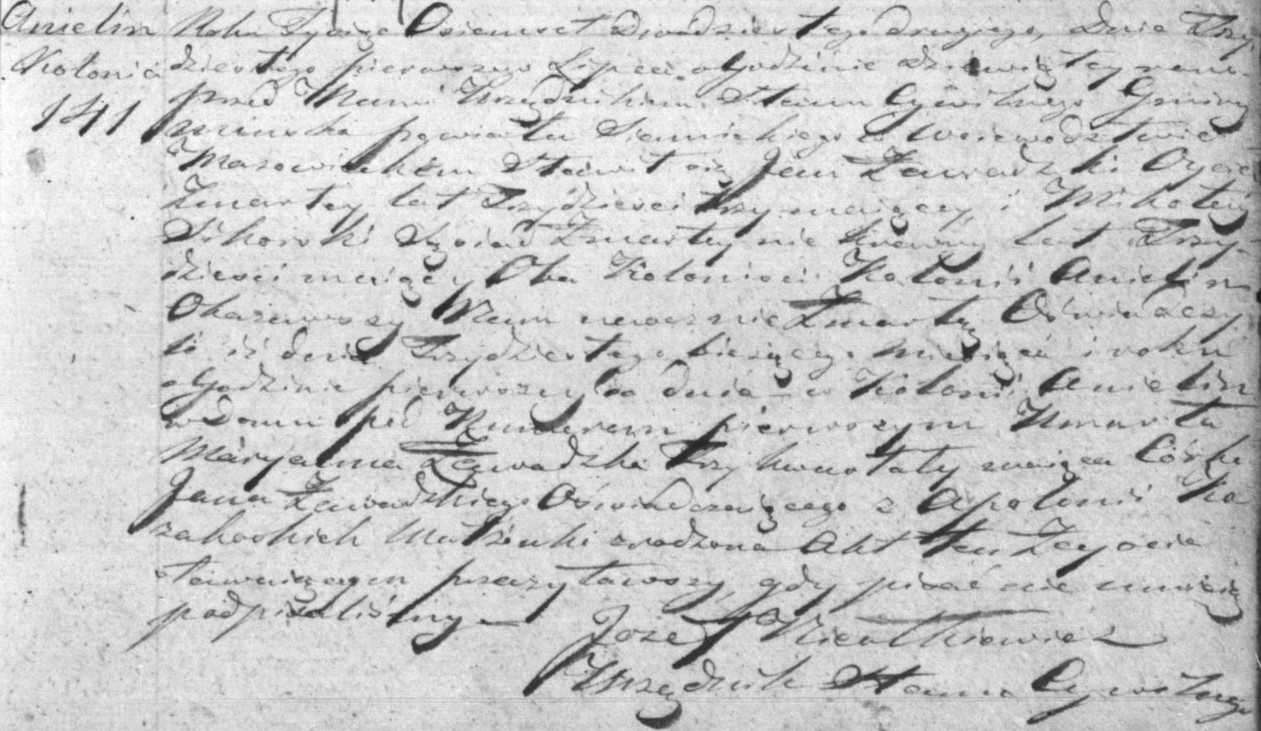
\includegraphics[width=1.0\linewidth]{
        Anielina_1822.jpg}
    \captionsetup{format=hang}
    \caption{Pierwszy znany wpis dotyczący wsi Anielina pochodzący 
    z~1822~roku z~akt stanu cywilnego gminy Mińsk Mazowiecki 
    \cite{par_minsk1}.}
    \label{fig:anielina_1822}
\end{figure}

Pierwszym dzieckiem Piotra i~Marianny Gumulskich, które urodziło się
w~Anielinie, a~zarazem ich czwartą córką, była Rozalia Gomulska. Urodziła się
ona 18~listopada 1853~roku, a~w~akcie jej chrztu jej ojciec został określony 
jako gospodarz mający 38~lat zamieszkały we wsi Angelina. Rodzicami chrzestymi 
Rozalii Gomulskiej zostali Władysław Michalski oraz Józefa Sadowska 
(patrz: ryc. \ref{fig:rgomulska_1853}).

\begin{figure}[!ht]
    \vspace*{0.5cm}
    \centering \includegraphics[width=1.0\linewidth]{
        1853_Rozalia_Gomulska_Szostak_akt_chrztu_parafia_Mińsk_Mazowiecki_wpis_260.jpg}
    \captionsetup{format=hang}
    \caption{Akt chrztu Rozalii Gomulskiej - par. Mińsk Mazowiecki 1851~rok 
    (260/1853) \cite{par_minsk2}.}
    \label{fig:rgomulska_1853}
\end{figure}

Dnia 7~października 1857~roku urodziła się najmłodsza córka Piotra i~Marianny
Gumulskich - Józefa Gomulska. W akcie jej chrztu, jej ojciec został określony 
jako \enquote{... kowal, lat czerdzieści pieć liczący, w Angelinie
zamieszkały...}. Rodzicami chrzestnymi Józefy Gomulskiej zostali Wojciech
Chłopik oraz Marianna Zawadzka (patrz: ryc. \ref{fig:jgomulska_1857}). We 
wrześniu 1859~roku we wsi Anielina na świat przyszedł Michał Gomulski, 
przedostatni syn małżeństwa Gumulskich, a~zarazem jeden z~trzech członków
rodziny Gomulskich, którzy byli założycielami wsi Desna (a~zarazem 
udziałowcami spółki \enquote{Desna}) - bezpośredni potomkowie Michała 
Gomulskiego mieszkają na Deśnie do dnia dzisiejszego, nosząc nazwisko po 
swoim przodku. W~akcie chrztu Michała jego ojciec ponownie zostal określony 
jako kowal z~Angeliny. Rodzicami chrzestnymi Michała Gomulskiego zostali Jan 
Ostrowski oraz Anna Wójcik (patrz: ryc. \ref{fig:mgomulski_1859}). 

\begin{figure}[!ht]
    \vspace*{0.5cm}
    \centering 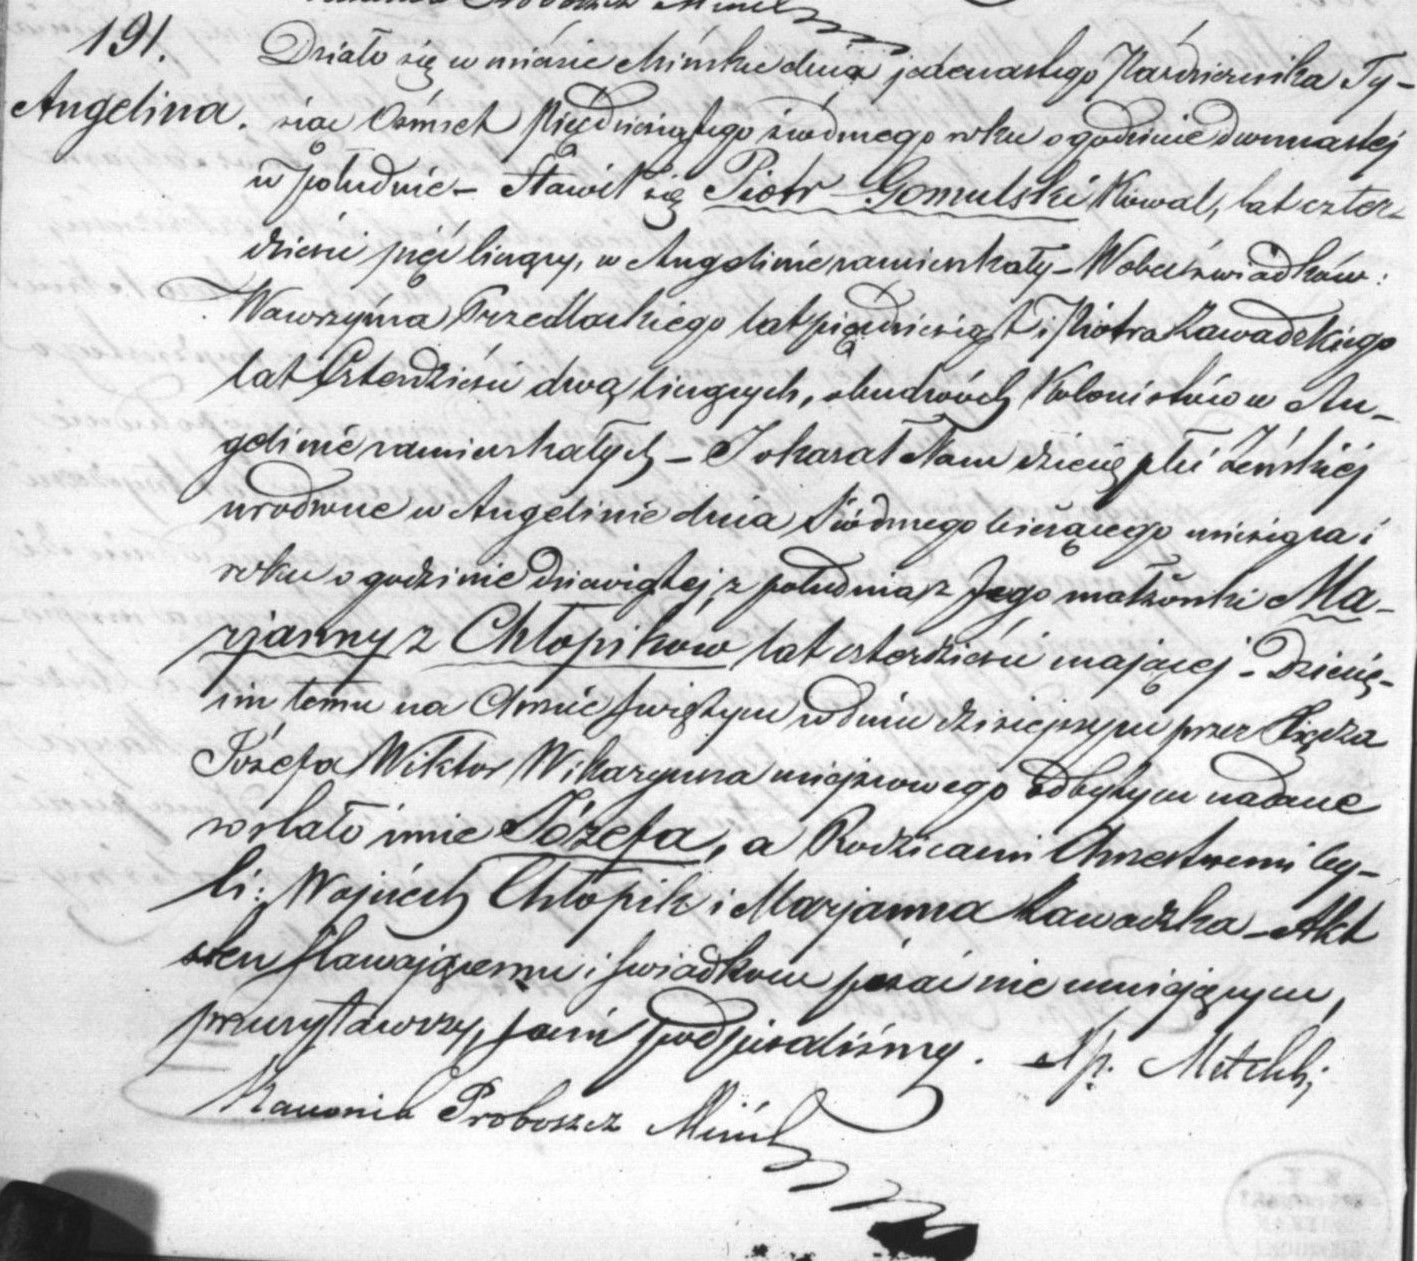
\includegraphics[width=1.0\linewidth]{
        1857_Józefa_Gomulska_akt_chrztu_parafia_Mińsk_Mazowiecki_wpis_191.jpg}
    \captionsetup{format=hang}
    \caption{Akt chrztu Józefy Gomulskiej - par. Mińsk Mazowiecki 1857~rok 
    (191/1857) \cite{par_minsk2}.}
    \label{fig:jgomulska_1857}
\end{figure}

Ostatnim dzieckiem Piotra i~Marianny Gumulskich był Stanisław Gomulski 
urodzony w~Anielinie 2~listopada 1863~roku. W~momencie jego narodzin jego 
rodzice mieli odpowiednio 48~lat (ojciec) oraz 44~lata (matka). Ojciec 
Stanisława w~akcie jego chrztu został określony jako kolonista zamieszkały 
w~Angelinie\footnote{W tamtym czasie kolonistami nazywani byli nowo przybyli 
do danej miejscowości osadnicy.}. Rodzicami chrzestnymi Stanisława Gomulskiego 
zostali Władysław Michalski oraz Katarzyna Bodzionek (patrz: ryc. 
\ref{fig:sgomulski_1863}). Stanisław, podobnie jak jego cztery lata starszy 
brat Michał, był jedynym z~założycieli wsi Desna - bezpośredni potomkowie 
Stanisława Gomulskiego mieszkają na Deśnie do dnia dzisiejszego, ale nie 
noszą oni już nazwiska swojego przodka. Piotr i~Marianna Gumulscy mieli 
łącznie jedenaścioro dzieci, z~czego tylko sześcioro dożyło dorosłości, byli 
nimi: Jan (ur. 1836~r. - zm. 1901~r.), Grzegorz (ur. 1840~r. - zm. 1906~r.), 
Anna (ur. 1843~r. - zm. 1905~r.), Rozalia (ur. 1853~r. - zm. 1929~r.), Michał 
(ur. 1859~r. - zm. 1918~r.) i~Stanisław (ur. 1863~r. - zm. 1929~r.).

\begin{figure}[!ht]
    \vspace*{0.5cm}
    \centering 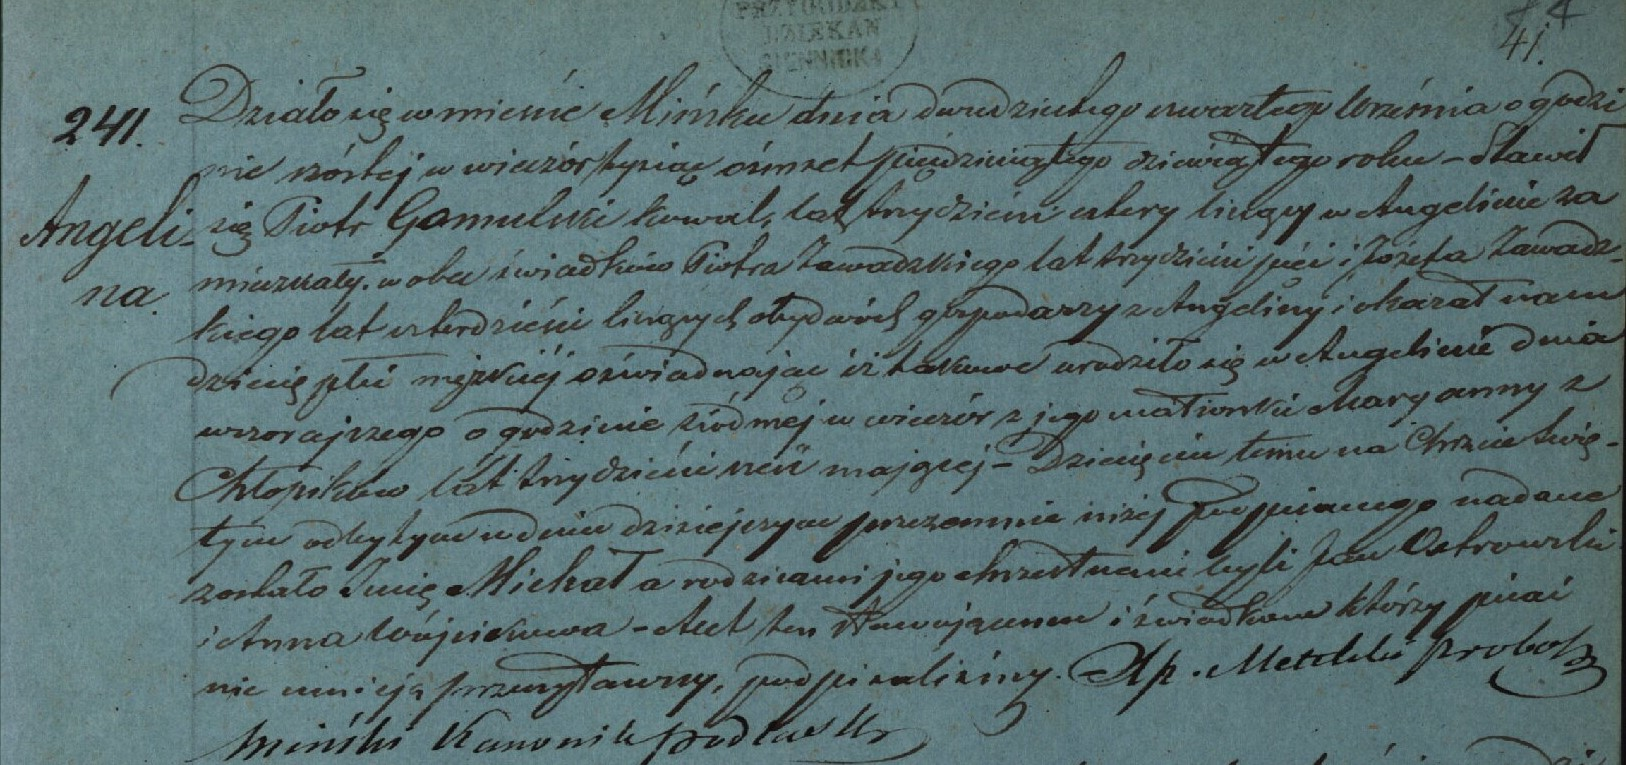
\includegraphics[width=1.0\linewidth]{
        1859_Michał_Gomulski_akt_chrztu_parafia_Mińsk_Mazowiecki_wpis_241.jpg}
    \captionsetup{format=hang}
    \caption{Akt chrztu Michała Gomulskiego - par. Mińsk Mazowiecki 1859~rok 
    (241/1859) \cite{par_minsk2}.}
    \label{fig:mgomulski_1859}
\end{figure}

\begin{figure}[!ht]
    \vspace*{0.5cm}
    \centering 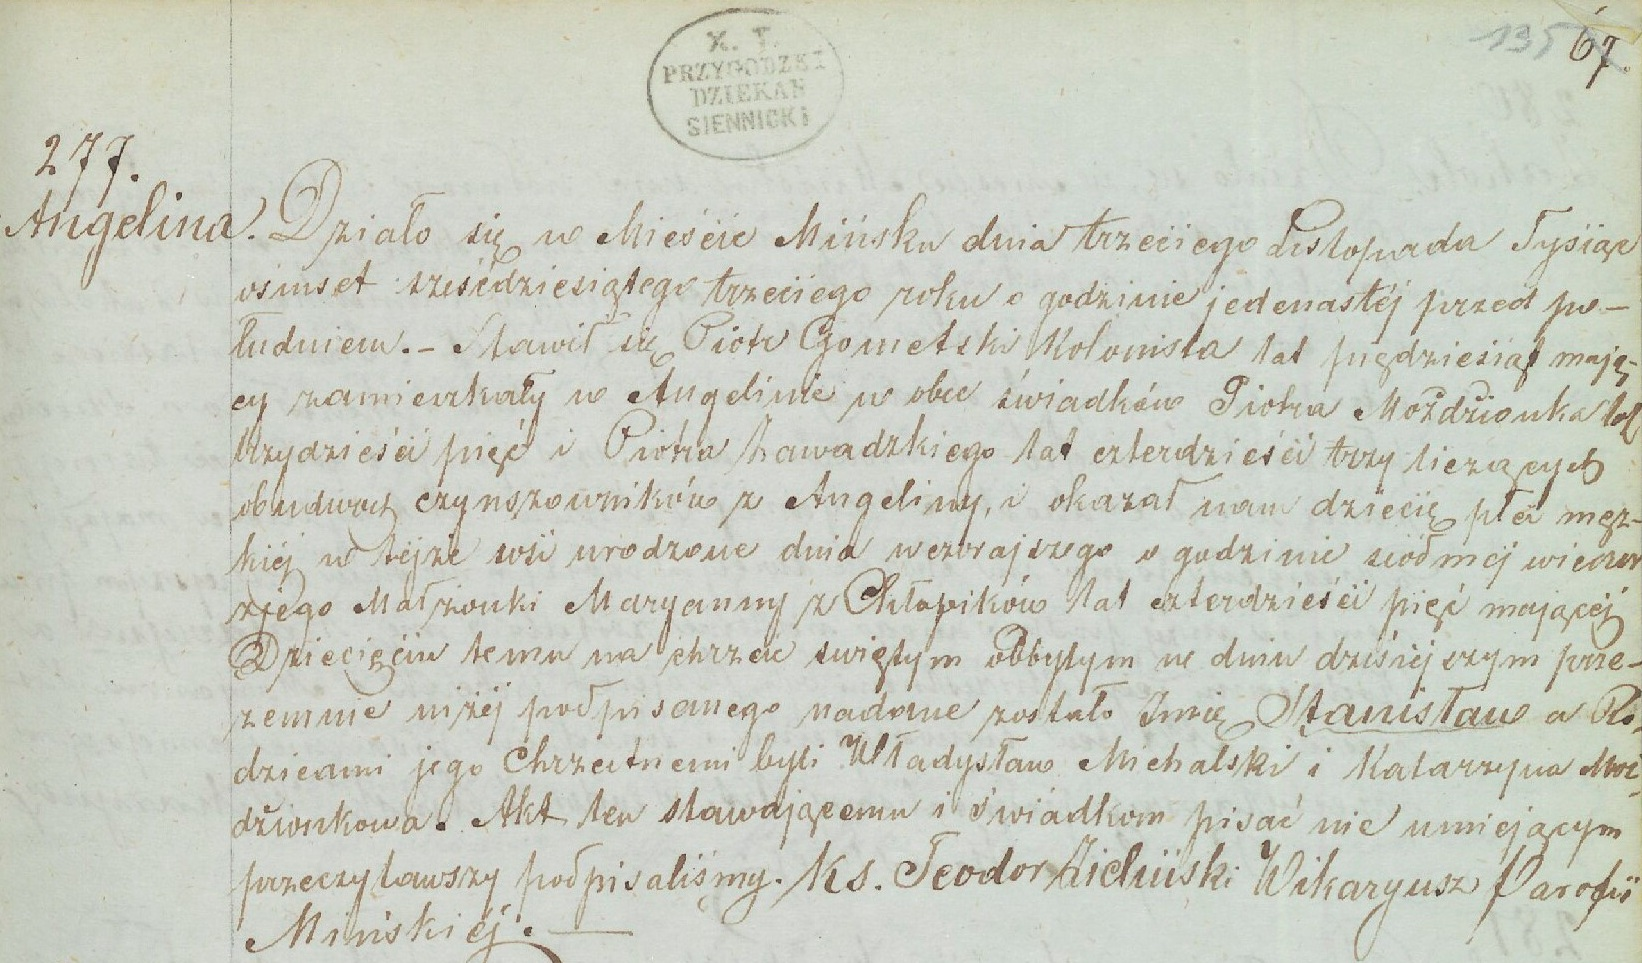
\includegraphics[width=1.0\linewidth]{
        1863_Stanisław_Gomulski_akt_chrztu_parafia_Mińsk_Mazowiecki_wpis_277.jpg}
    \captionsetup{format=hang}
    \caption{Akt chrztu Stanisława Gomulskiego - par. Mińsk Mazowiecki 
    1863~rok (277/1863) \cite{par_minsk2}.}
    \label{fig:sgomulski_1863}
\end{figure}

Piotr Franciszek Gumulski ostanie 17~lat swojego życia przeżył we wsi Anielina
 - zmarł 8~lutego 1870~roku w~wieku 55 lat (patrz: ryc.
 \ref{fig:pfgomulski_1870}\footnote{Akt zgonu Piotra Franciszka Gumulskiego 
 został sporządzony w~języku rosyjskim, gdyż począwszy od 1868~roku w~wyniku 
represji carskich po powstaniu styczniowym, wszystkie kościelne akta 
metrykalne w~Królestwie Polskim musiały być prowadzone w~języku rosyjskim - 
represje te były utrzymywane aż do 1915~roku.}). 

\begin{figure}[!ht]
    \vspace*{0.5cm}
    \centering \includegraphics[width=1.0\linewidth]{
        1870_Piotr_Franciszek_Gumulski_akt_zgonu_parafia_Mińsk_Mazowiecki_wpis_51.jpg}
    \captionsetup{format=hang}
    \caption{Akt zgonu Piotra Franciszka Gumulskiego - par. Mińsk Mazowiecki 
    1870~rok (51/1870) \cite{par_minsk2}.}
    \label{fig:pfgomulski_1870}
\end{figure}

\begin{figure}[!ht]
    \vspace*{0.5cm}
    \centering 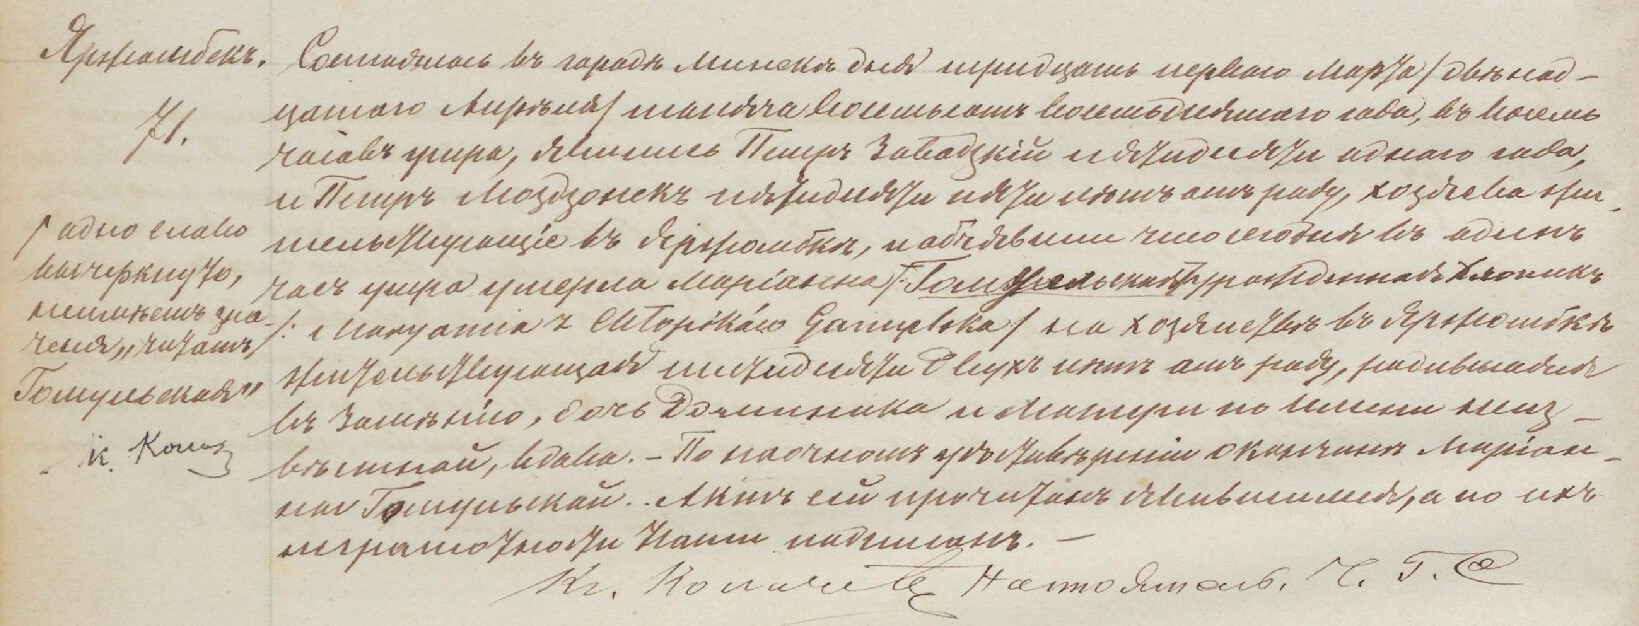
\includegraphics[width=1.0\linewidth]{
        1880_Marianna_Gumulska_Chłopik_akt_zgonu_parafia_Mińsk_Mazowiecki_wpis_71.jpg}
    \captionsetup{format=hang}
    \caption{Akt zgonu Marianny Gumulskiej - par. Mińsk Mazowiecki 
    1880~rok (71/1880) \cite{par_minsk2}.}
    \label{fig:mgomulska_1880}
\end{figure}

Marianna Gumulska (z~domu Chłopik) zmarła 10~lat po swoim mężu - 12~kwietnia 
1880~roku, dożywając wieku 61~lat. W~akcie jej zgonu wskazano, iż 
zmarła ona we wsi Jarząbek, czyli pobliskiej w~stosunku do Anieliny wsi, do 
której Marianna prawdopodobnie przeprowadziła się  ze swoim szwagrem oraz jego
 rodziną (patrz: ryc. \ref{fig:mgomulska_1880}).

\begin{figure}[!ht]
    \vspace*{0.5cm}
    \centering 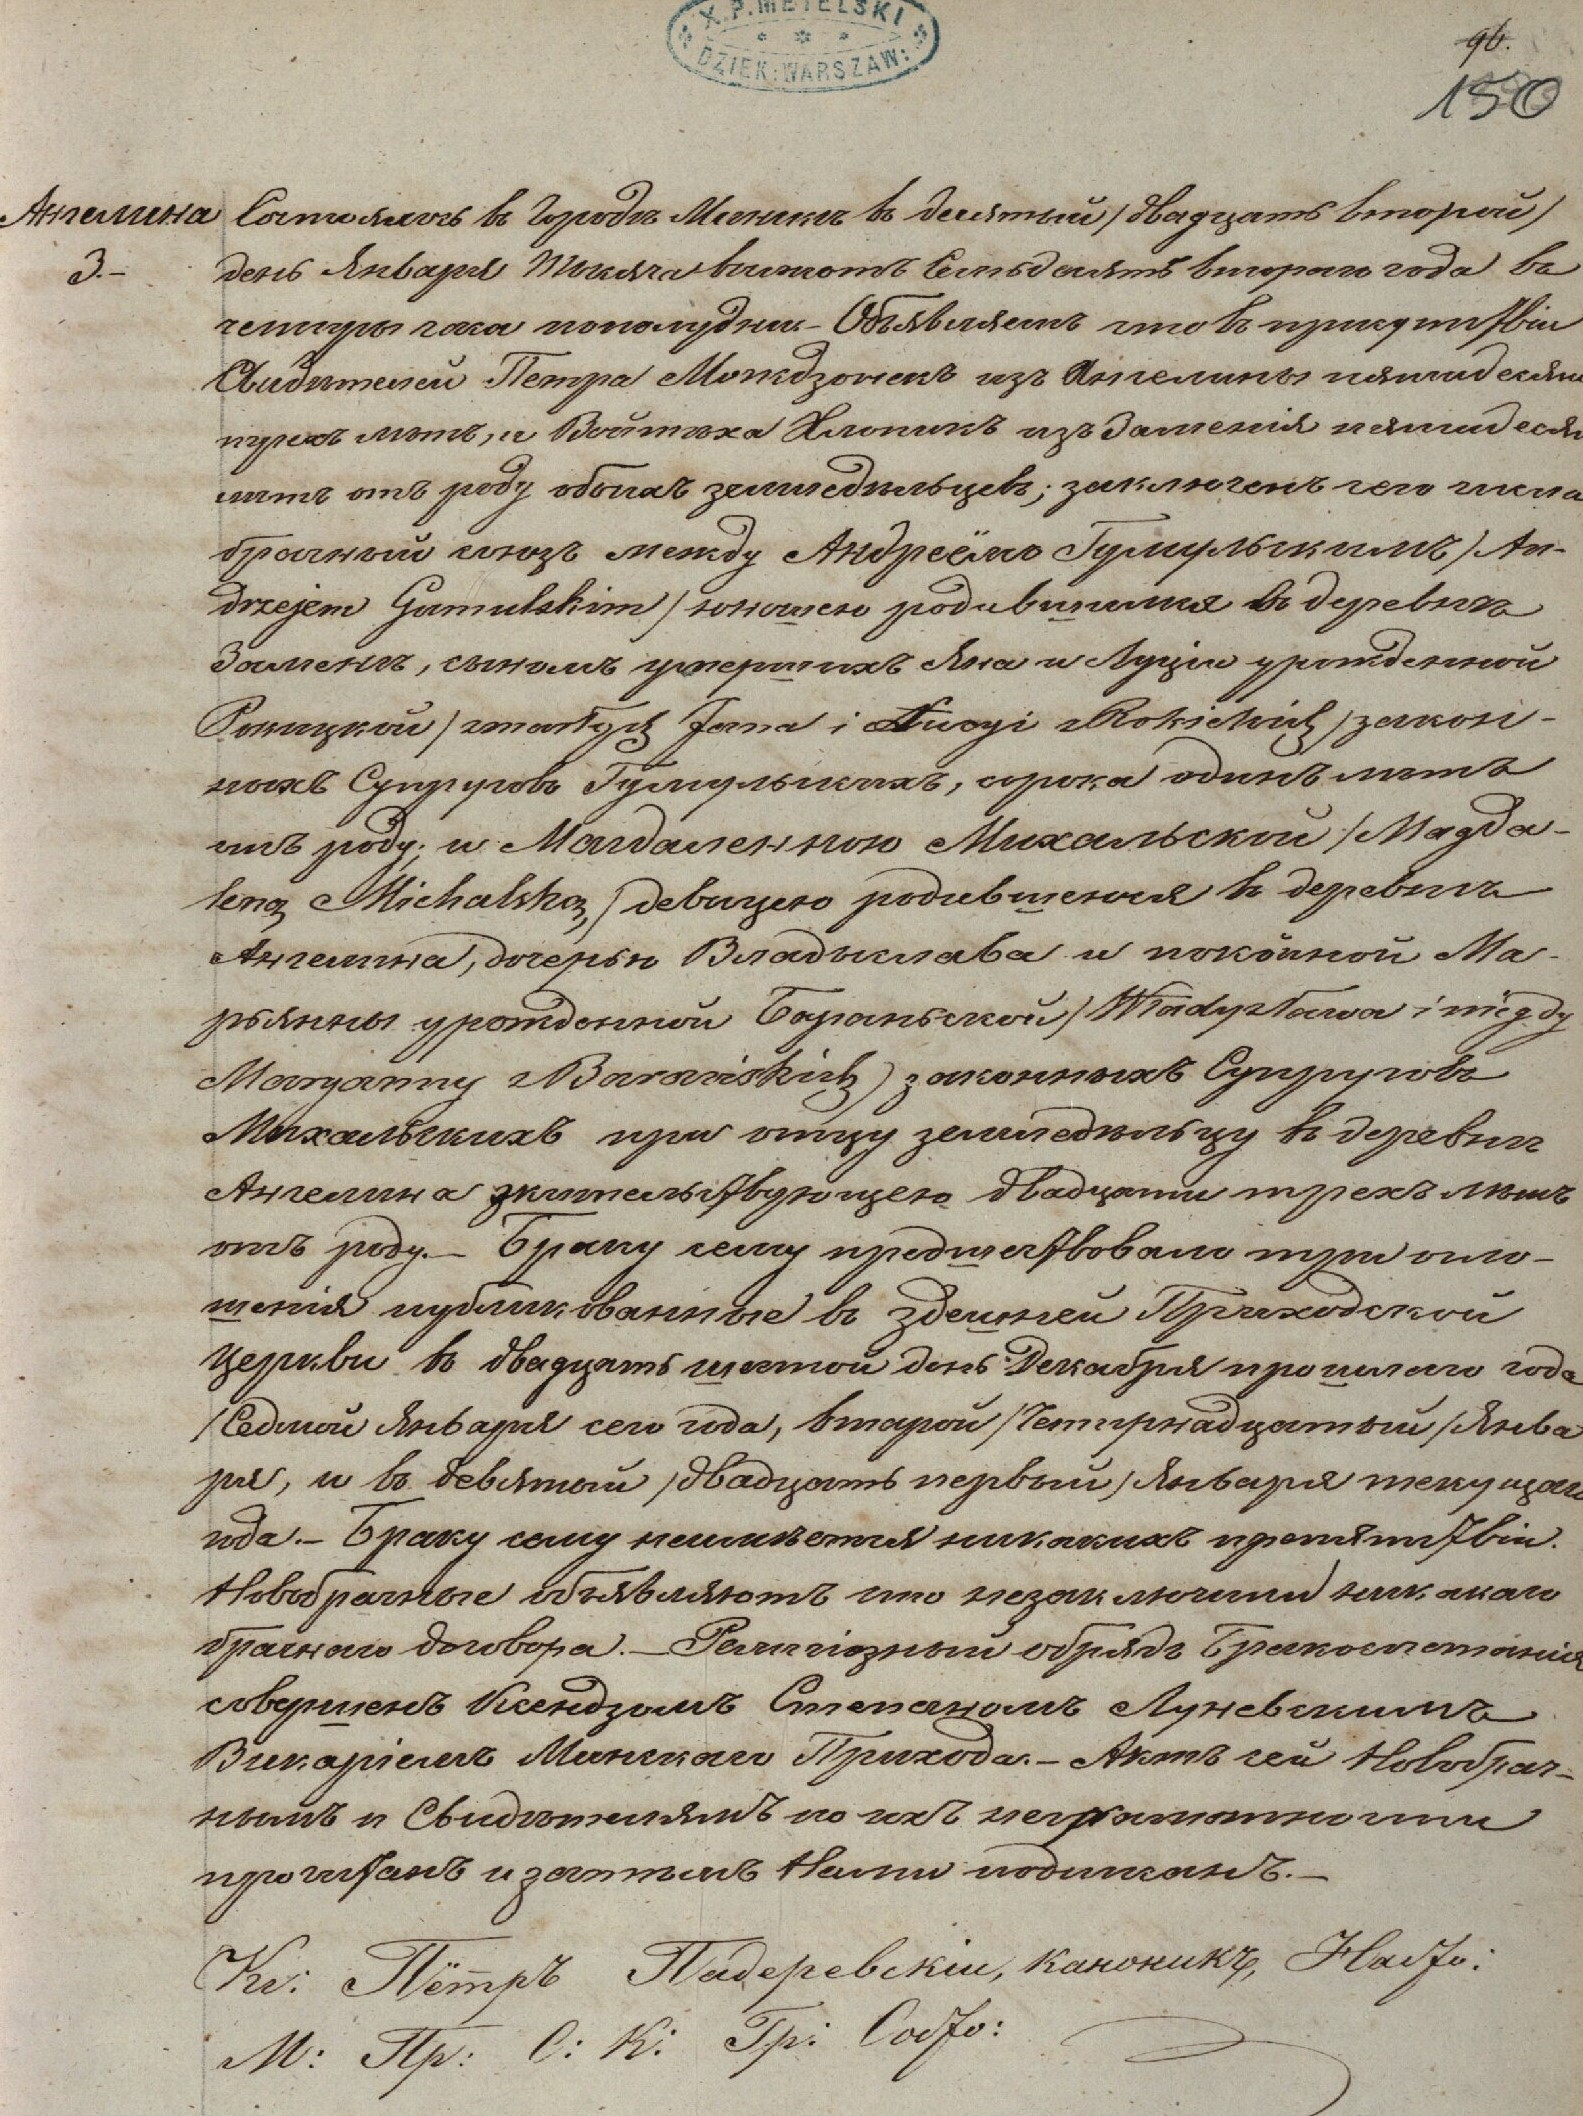
\includegraphics[width=0.92\linewidth]{
        1872_Andrzej_Gomulski_Magdalena_Michalska_akt_ślubu_parafia_Mińsk_Mazowiecki_wpis_3.jpg}
    \captionsetup{format=hang}
    \caption{Akt ślubu Andrzeja Gumulskiego i~Magdaleny Michalskiej - par. 
    Mińsk Mazowiecki 1872~rok (3/1872) \cite{par_minsk2}.}
    \label{fig:agumulski_1872}
\end{figure}

Około 1872~roku, dwa lata po śmierci Piotra Gumulskiego, do Anieliny 
przeprowadził się jego młodszy brat Andrzej. Powodem jego przeprowadzki do 
Anielny był prawdopodobnie ślub, który wziął z~lokalną dziewczyną, Magdaleną 
Michalską, 22~stycznia 1872~roku w~Mińsku Mazowieckim. Andrzej Gumulski miał 
wówczas blisko 42~lata, a~jego przyszła żona ledwo ukończyła 23 lata (patrz: 
ryc. \ref{fig:agumulski_1872}). 

  \begin{figure}[!ht]
    \vspace*{0.5cm}
    \centering \includegraphics[width=1.0\linewidth]{
        1875_Feliks_Gomulski_akt_chrztu_parafia_Mińsk_Mazowiecki_wpis_126.jpg}
    \captionsetup{format=hang}
    \caption{Akt chrztu Feliksa Gomulskiego - par. Mińsk Mazowiecki 
    1875~rok (126/1875) \cite{par_minsk2}.}
    \label{fig:fgomulski_1875}
\end{figure}

Andrzej Gumulski wraz ze swoją żoną Magdaleną dochowali się trójki dzieci, 
z~czego dwójka najstarszych urodziła się w~Anielinie, a trzecie z~nich 
urodziło się we wsi Jarząbek: 

\begin{itemize}
    \item Feliks Gomulski (ur. 1875~r. - zm. 1941~r.) - patrz: ryc. 
    \ref{fig:fgomulski_1875},
    \item Antonina Gomulska (ur. 1878~r. - zm. 1955~r.) - patrz: ryc. 
    \ref{fig:agomulska_1878},
    \item Józefę (ur. 1882~r. - zm. 1884~r.)  - patrz: ryc. 
    \ref{fig:lgomulska_1882} oraz ryc. \ref{fig:lgomulska_1884}.
  \end{itemize}

Wygląda więc na to, że Andrzej Gumulski wraz z~żoną, dziećmi oraz 
bratową Marianną przeprowadzili się do Jarząbka około 1880~roku, jednak po 
1884~roku wrócili do Anieliny, bo tam zmarł zarówno Andrzej - w~1887~roku 
(patrz: ryc. \ref{fig:agomulski_1887}), jak i jego żona Magdalena - 
w~1904~roku.

\begin{figure}[!ht]
    \vspace*{0.5cm}
    \centering 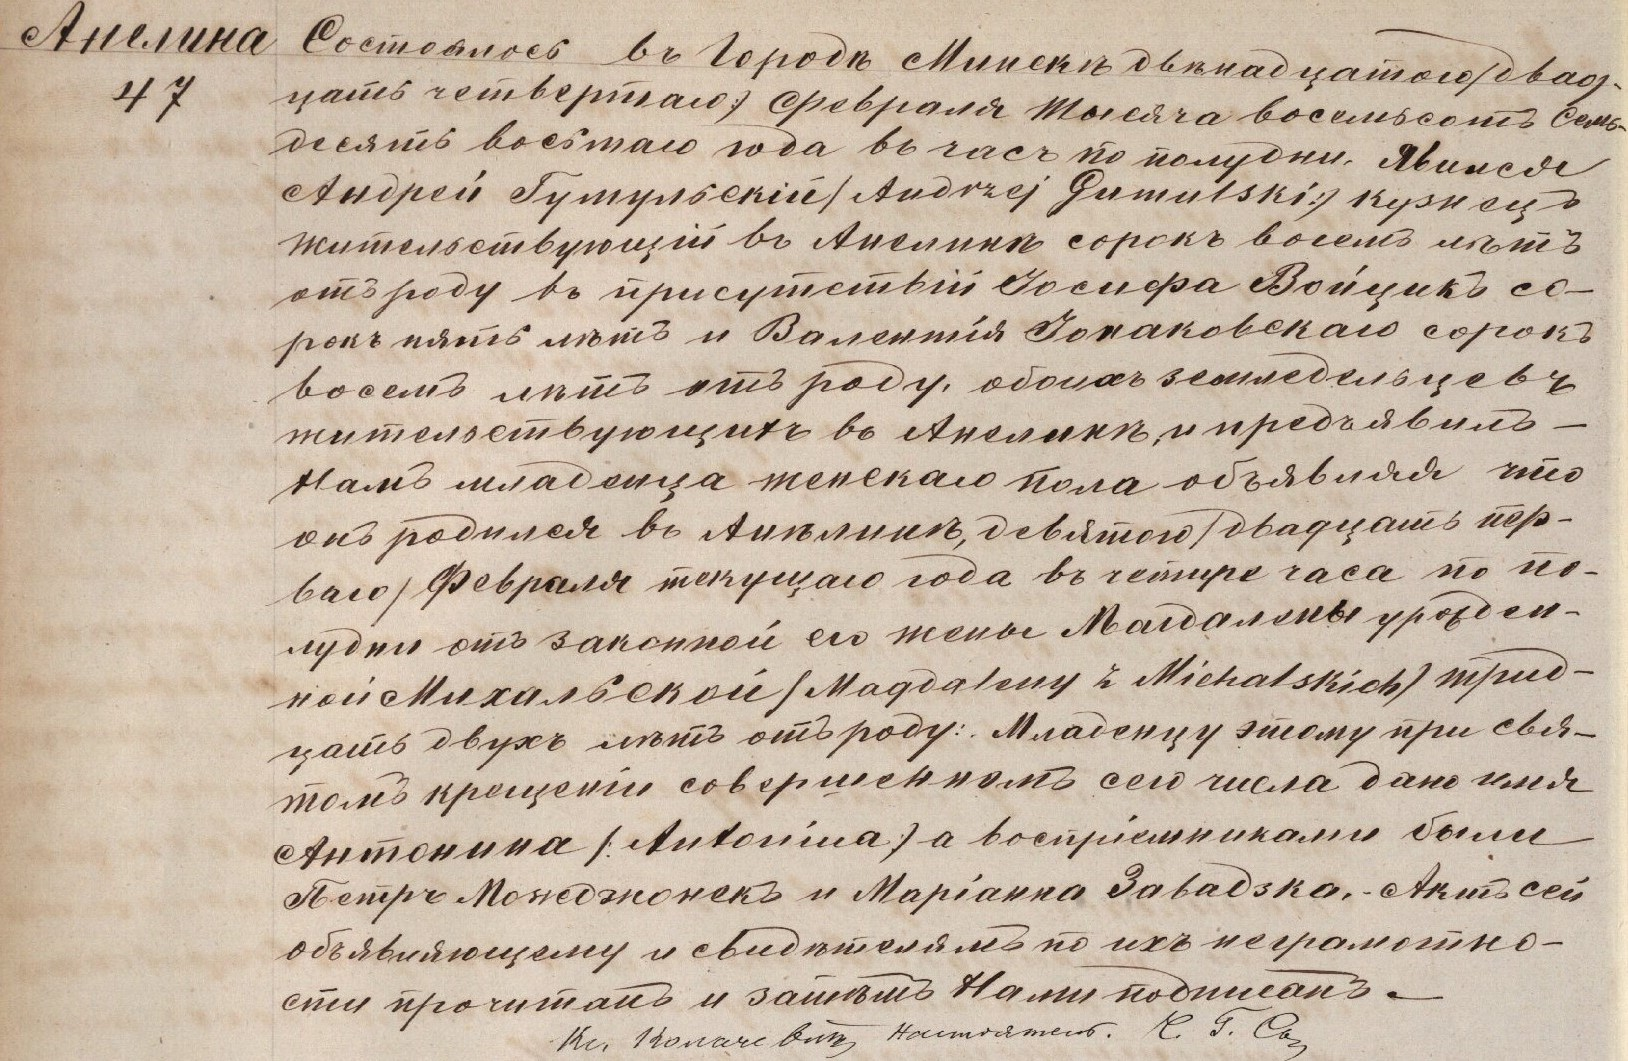
\includegraphics[width=0.99\linewidth]{
        1878_Antonina_Gomulska_Araźna_akt_chrztu_parafia_Mińsk_Mazowiecki_wpis_47.jpg}
    \captionsetup{format=hang}
    \caption{Akt chrztu Antoniny Gomulskiej - par. Mińsk Mazowiecki 
    1878~rok (47/1878) \cite{par_minsk2}.}
    \label{fig:agomulska_1878}
\end{figure}

\begin{figure}[!ht]
    \vspace*{0.5cm}
    \centering \includegraphics[width=0.99\linewidth]{
        1882_Ludwika_Gomulska_akt_chrztu_parafia_Mińsk_Mazowiecki_wpis_167.jpg}
    \captionsetup{format=hang}
    \caption{Akt chrztu Ludwiki Gomulskiej - par. Mińsk Mazowiecki 
    1882~rok (167/1882) \cite{par_minsk2}.}
    \label{fig:lgomulska_1882}
\end{figure}

\begin{figure}[!ht]
    \vspace*{0.5cm}
    \centering \includegraphics[width=0.93\linewidth]{
        1884_Ludwika_Gomulska_akt_zgonu_parafia_Mińsk_Mazowiecki_wpis_70.jpg}
    \captionsetup{format=hang}
    \caption{Akt zgonu Ludwiki Gomulskiej - par. Mińsk Mazowiecki 
    1884~rok (70/1884) \cite{par_minsk2}.}
    \label{fig:lgomulska_1884}
\end{figure}

\begin{figure}[!ht]
    \vspace*{0.5cm}
    \centering \includegraphics[width=0.93\linewidth]{
        1887_Andrzej_Gomulski_akt_zgonu_parafia_Mińsk_Mazowiecki_wpis_13.jpg}
    \captionsetup{format=hang}
    \caption{Akt zgonu Andrzeja Gumulskiego - par. Mińsk Mazowiecki 
    1887~rok (13/1887) \cite{par_minsk2}.}
    \label{fig:agomulski_1887}
\end{figure}

Z trójki dzieci Andrzeja i~Magdaleny Gumulskich tylko dwójka dożyła wieku 
dorosłego - Feliks Gomulski ożenił się w~1909~roku w~Pęcicach pod Pruszkowem 
z~Małgorzatą Makowską pochodzącą ze Słomina (patrz: ryc. 
\ref{fig:fgomulski_1909}) a~Antonina Gomulska w~1896~roku wyszła za mąż 
w~Mińsku Mazowieckim za Michała Araźnego pochodzącego ze wsi Olesin, 
znajdującej się koło Dębego Wielkiego.

\begin{figure}[!ht]
    \vspace*{0.5cm}
    \centering 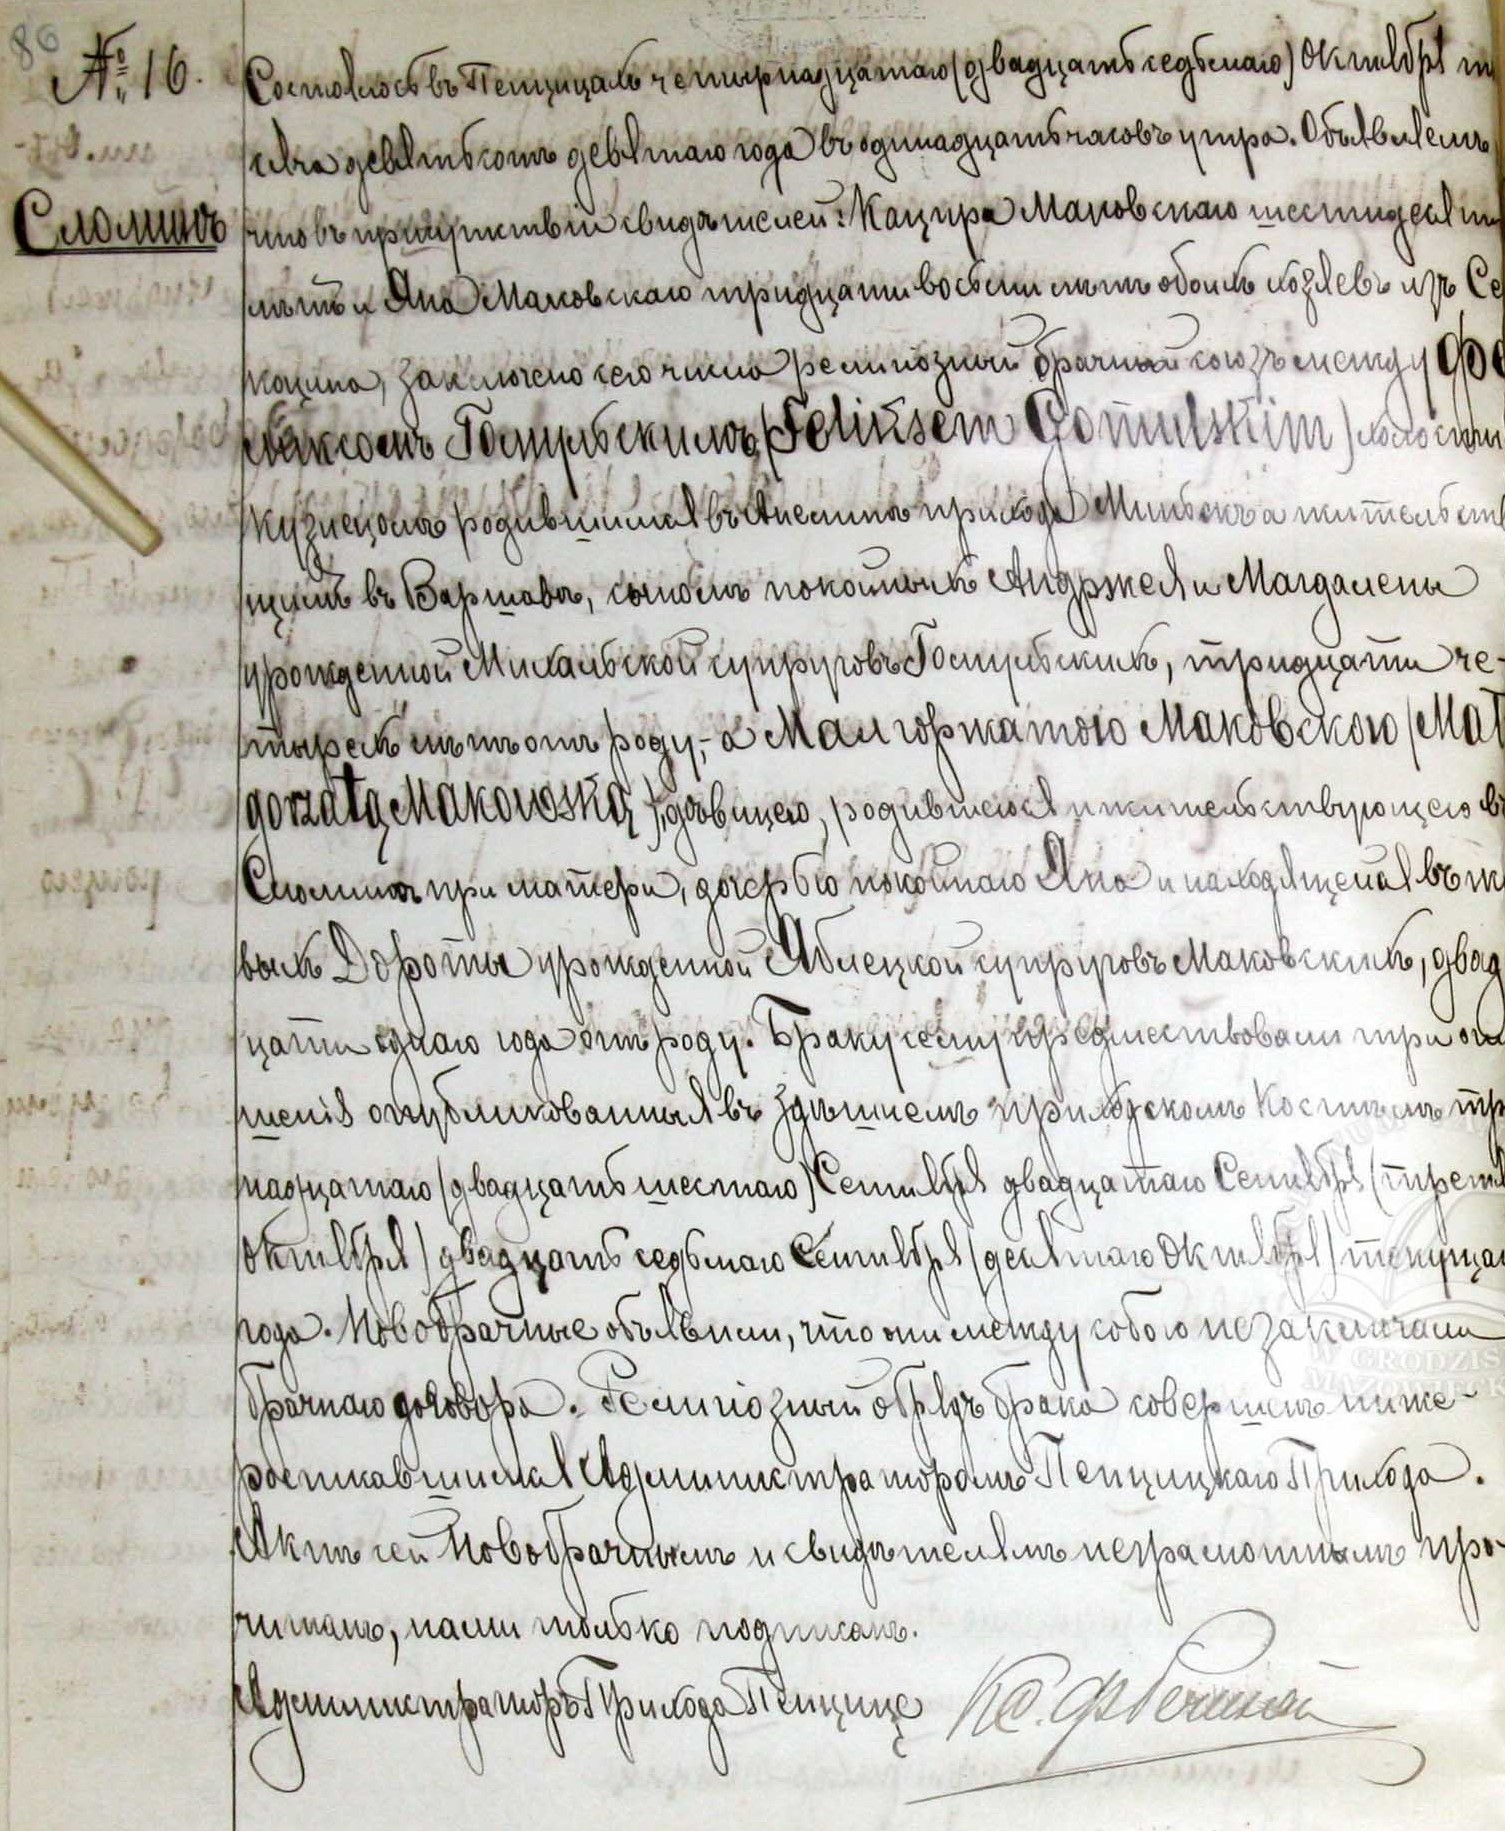
\includegraphics[width=1.0\linewidth]{
        1909_Feliks_Gomulski_Małgorzata_Makowska_akt_ślubu_parafia_Pęcice_wpis_16.jpg}
    \captionsetup{format=hang}
    \caption{Akt ślubu Feliksa Gomulskiego oraz Małgorzaty Makowskiej - par. 
    Pęcice 1909~rok (16/1909) \cite{par_pecice}.}
    \label{fig:fgomulski_1909}
\end{figure}

\begin{figure}[!ht]
    \vspace*{0.5cm}
    \centering \includegraphics[width=0.8\linewidth]{
        1910_Henryk_Gomulski_akt_chrztu_parafia_Pęcice_wpis_77.jpg}
    \captionsetup{format=hang}
    \caption{Akt chrztu Henryka Gomulskiego - par. Pęcice 1910~rok (77/1910) 
    \cite{par_pecice}.}
    \label{fig:hgomulski_1910}
\end{figure}

\begin{figure}[!ht]
    \vspace*{0.5cm}
    \centering 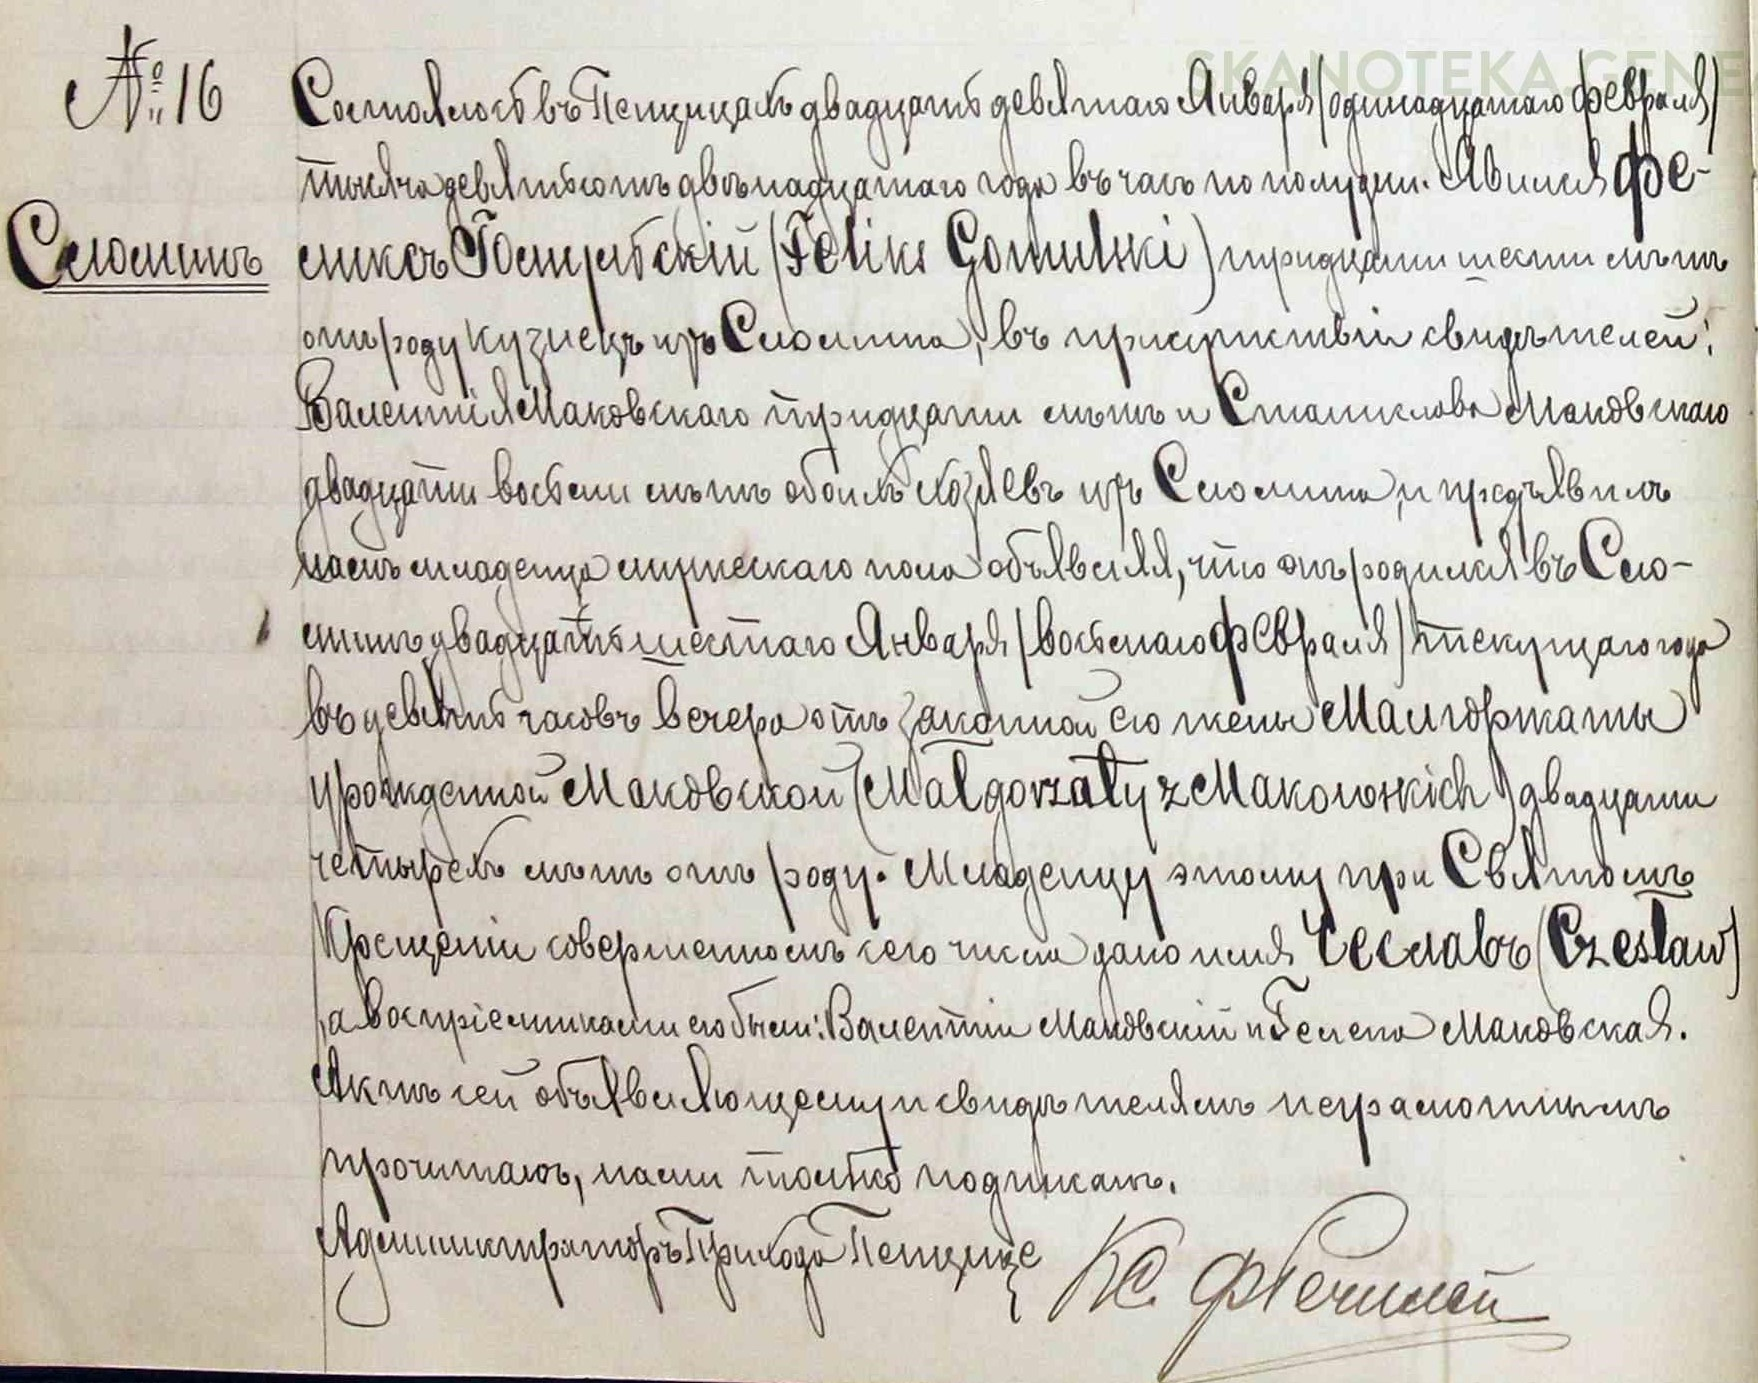
\includegraphics[width=0.8\linewidth]{
        1912_Czesław_Gomulski_akt_chrztu_parafia_Pęcice_wpis_16.jpg}
    \captionsetup{format=hang}
    \caption{Akt chrztu Czesława Gomulskiego - par. Pęcice 1912~rok (16/1912) 
    \cite{par_pecice}.}
    \label{fig:czgomulski_1912}
\end{figure}

Feliks Gomulski razem ze swoją małżonką przez pierwsze kilka lat po ślubie 
mieszkali w~rodzinej wsi Małgorzaty - w~Słominie, o~czym świadczy fakt, iż 
ich dwóch pierwszych synów Henryk (patrz: ryc. \ref{fig:hgomulski_1910}) oraz 
Czesław (patrz: ryc. \ref{fig:czgomulski_1912}) urodziło się (odpowiednio 
w~1910 oraz 1912~roku) właśnie w~tej miejscowości. Trzeci syn małżeństwa 
Gomulskich, Walerian (patrz: ryc. \ref{fig:wgomulski_1914}), urodził się 
w~1914~roku w~Mińsku Mazowieckim, a~ich pierwsza córka, Helena, urodziła 
się (patrz: ryc. \ref{fig:hgomulska_1917}) oraz zmarła (patrz: ryc. 
\ref{fig:hgomulska_1917_2}) w~1917~roku w~Anielinie. Oznacza to, że po około 
8~latach od ślubu, Feliks Gomulskich powrócił do swojej rodzinnej 
miejscowości.

\begin{figure}[!ht]
    \vspace*{0.5cm}
    \centering \includegraphics[width=0.9\linewidth]{
        1914_Walerian_Gomulski_akt_chrztu_parafia_Mińsk_Mazowiecki_wpis_674.jpg}
    \captionsetup{format=hang}
    \caption{Akt chrztu Waleriana Gomulskiego - par. Mińsk Mazowiecki 
    1914~rok (674/1914) 
    \cite{par_minsk2}.}
    \label{fig:wgomulski_1914}
\end{figure}

\begin{figure}[!ht]
    \vspace*{0.5cm}
    \centering \includegraphics[width=1.0\linewidth]{
        1917_Helena_Gomulska_akt_chrztu_parafia_Mińsk_Mazowiecki_wpis_50.jpg}
    \captionsetup{format=hang}
    \caption{Akt chrztu Heleny Gomulskiej - par. Mińsk Mazowiecki 
    1917~rok (50/1917) 
    \cite{par_minsk2}.}
    \label{fig:hgomulska_1917}
\end{figure}

Czwarty syn małżeństwa Gomulskich, Zygmunt, urodził się również 
w~Anielinie, w~1918~roku (patrz: ryc. \ref{fig:zgomulski_1918}), natomiast 
ich druga córka, Janina, podobnie jak jej starszy brat Walerian, urodziła się 
w~Mińsku Mazowieckim, w~1920~roku (patrz: ryc. \ref{fig:jgomulska_1920}). Co 
ciekawe, w~aktach chrztu Heleny, Zygmunta oraz Janiny, ich ojciec, Feliks 
Gomulski określony został jako kowal, w~dwóch pierwszych wskazano, iż 
zamieszkuje on w~Anielinie natomiast w~trzecim, jako jego miejscowość 
zamieszkania wskazano Grzebowilk. Oznacza to, iż Feliks Gomulski, kontynuował 
rodzinną tradycję i~podobnie jak jego ojciec i~dziadek trudnił się pracą 
kowala w~miejscowościach, w~których zamieszkiwał.

\begin{figure}[!ht]
    \vspace*{0.5cm}
    \centering \includegraphics[width=1.0\linewidth]{
        1918_Zygmunt_Gomulski_akt_chrztu_parafia_Mińsk_Mazowiecki_wpis_196.jpg}
    \captionsetup{format=hang}
    \caption{Akt chrztu Zygmunta Gomulskiego - par. Mińsk Mazowiecki 
    1918~rok (196/1918) 
    \cite{par_minsk2}.}
    \label{fig:zgomulski_1918}
\end{figure}

Autor niniejszej książki nie dysponuje informacjami na temat miejsca narodzin, 
dwóch najmłodszych dzieli Feliksa i Magdaleny Gomulskich - Jadwigi 
i~Mieczysława, gdyż w~momencie pisania niniejszej książki, kościelne akta 
chrztów dostępne do publicznego wglądu, kończyły się, w~zależności od 
parafii, na około 1920~roku\footnote{Większość archidiecezji w~Polsce nie 
udostępnia do publicznego wglądu aktów chrztów młodszych niż 100~lat oraz 
aktów ślubów i~zgonów młodszych niż 80~lat - ze względu na prywatność danych 
osobowych.}. Na podstawie grobów rodziny Gomulskich, znajdujących się na 
cmentarzu parafialnym parafii pod wezwaniem św. Kazimierza w~Pruszkowie, 
można jedynie stwierdzić, iż urodzili się oni odpowiednio w~1923 (patrz: ryc. 
\ref{fig:mgomulska_1951}) oraz w~1929~roku (patrz: ryc. 
\ref{fig:czgomulski_1946}).

\begin{figure}[!ht]
    \vspace*{0.5cm}
    \centering \includegraphics[width=1.0\linewidth]{
        1920_Janina_Gomulska_akt_chrztu_parafia_Mińsk_Mazowiecki_wpis_347.jpg}
    \captionsetup{format=hang}
    \caption{Akt chrztu Janiny Gomulskiej - par. Mińsk Mazowiecki 
    1920~rok (347/1920) 
    \cite{par_minsk2}.}
    \label{fig:jgomulska_1920}
\end{figure}

\begin{figure}[!ht]
    \vspace*{0.5cm}
    \centering \includegraphics[width=1.0\linewidth]{
        1917_Helena_Gomulska_akt_zgonu_parafia_Mińsk_Mazowiecki_wpis_303.jpg}
    \captionsetup{format=hang}
    \caption{Akt zgonu Heleny Gomulskiej - par. Mińsk Mazowiecki 
    1917~rok (303/1917) 
    \cite{par_minsk2}.}
    \label{fig:hgomulska_1917_2}
\end{figure}


Feliks i~Małgorzata Gomulscy, jak można wywnioskować na podstawie aktów 
chrztów ich dzieci, bardzo często zmieniali miejsca swojego zamieszkania. 
Były to często przeprowadzki na odległości kilkudziesięciu kilometrów, 
z~jednej strony Warszawy na drugą. Wygląda na to, że w~latach 30. XX wieku 
przeprowadzili się ostatecznie razem z~dziećmi do Pruszkowa, gdzie żyli do 
końca swoich dni - jak wynika z~informacji znajdujących się na ich nagrobkach, 
Feliks Gomulski zmarł w~1941~roku (patrz: ryc. \ref{fig:fgomulski_1941}), 
natomiast jego żona Małgorzata z~Makowskich zmarła w~1951~roku (patrz: ryc. 
\ref{fig:mgomulska_1951}).

\begin{figure}[!ht]
    \vspace*{0.5cm}
    \centering 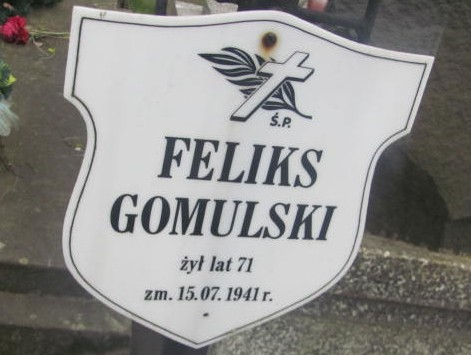
\includegraphics[width=0.9\linewidth]{
        1941_Feliks_Gomulski_zdjęcie_nagrobka1_cmentarz_Pruszków.jpg}
    \captionsetup{format=hang}
    \caption{Zdjęcie tablicy nagrobnej Feliksa Gomulskiego znajdującej się na
    cmentarzu parafialnym parafii pod wezwaniem św. Kazimierza w~Pruszkowie 
    (sektor: P2, rząd: 2, numer: 59)}
    \label{fig:fgomulski_1941}
\end{figure}

Dalsze losy dzieci Feliksa i~Małgorzaty Gomulskich nie są znane autorowi 
niniejszej książki. Jedyne informacje jakie udało się zdobyć, to te 
pochodzące z~nagrobków grobów znajdujących się na cmentarzu w~Pruszkowie,  
wskazują one, iż:

\begin{itemize}
    \item Zygmunt zmarł w~1943~roku (patrz: ryc. \ref{fig:zgomulski_1943}),
    \item Czesław zmarł w~1946~roku (patrz: ryc. \ref{fig:czgomulski_1946}),
    \item Mieczysław zmarł w~1968~roku (patrz: ryc. \ref{fig:czgomulski_1946}),
    \item Jadwiga zmarła w~1994~roku (patrz: ryc. \ref{fig:mgomulska_1951}),
    \item Walerian zmarł w~1995~roku (patrz: ryc. \ref{fig:mgomulska_1951}),
    \item Janina dożyła do 2008~roku\footnote{W~chwili śmierci Janina nosiła 
    nazwisko \emph{Kubiciel}, bo jak wynika z~notatki zamieszczonej na akcie 
    chrztu Janiny, w~1978~roku, wyszła ona za mąż za Wacława Kubiciela.} 
    (patrz: ryc. \ref{fig:zgomulski_1943}).
\end{itemize}

\begin{figure}[!ht]
    \vspace*{0.5cm}
    \centering 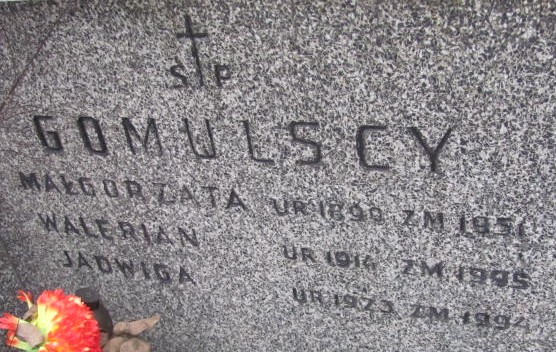
\includegraphics[width=0.87\linewidth]{
        1951_Małgorzata_Gomulska_Makowska_zdjęcie_nagrobka2_cmentarz_Pruszków.jpg}
    \captionsetup{format=hang}
    \caption{Zdjęcie grobu Małgorzaty, Waleriana i~Jadwigi Gomulskich 
    znajdującego się na cmentarzu parafialnym parafii pod wezwaniem św. 
    Kazimierza w~Pruszkowie (sektor: P4, rząd: 3, numer: 21)}
    \label{fig:mgomulska_1951}
\end{figure}

\begin{figure}[!ht]
    \vspace*{0.5cm}
    \centering 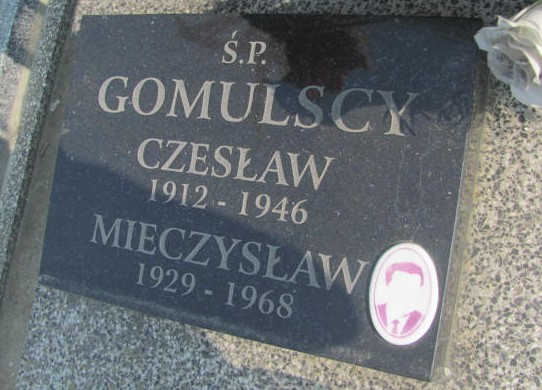
\includegraphics[width=0.87\linewidth]{
        1946_Czesław_Gomulski_zdjęcie_nagrobka1_cmentarz_Pruszków.jpg}
    \captionsetup{format=hang}
    \caption{Zdjęcie grobu Czesława i~Mieczysława Gomulskich znajdującego się 
    na cmentarzu parafialnym parafii pod wezwaniem św. Kazimierza 
    w~Pruszkowie (sektor: B3, rząd: 4, numer: 10)}
    \label{fig:czgomulski_1946}
\end{figure}

Co ciekawe, na stronie Muzeum Powstania Warszawskiego 
(\url{https://www.1944.pl}), widnieje informacja, iż Walerian Gomulski był 
uczestnikiem Powstania Warszawskiego, gdzie walczył w~stopniu strzelca, po 
czym trafił do niemieckiej niewoli - numer jeniecki: 45706\footnote{
Biogram Powstańczy: \url{https://www.1944.pl/powstancze-biogramy/walerian-gomulski,14633.html}}.

\begin{figure}[!ht]
    \vspace*{0.5cm}
    \centering 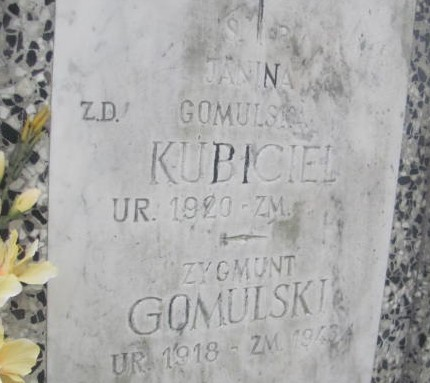
\includegraphics[width=0.7\linewidth]{
        1943_Zygmunt_Gomulski_zdjęcie_nagrobka2_cmentarz_Pruszków.jpg}
    \captionsetup{format=hang}
    \caption{Zdjęcie grobu Zygmunta Gomulskiego i~Janiny Kubiciel 
    znajdującego się na cmentarzu parafialnym parafii pod wezwaniem św. 
    Kazimierza w~Pruszkowie (sektor: P2, rząd: 6, numer: 37)}
    \label{fig:zgomulski_1943}
\end{figure}

Historia rodziny Gomulskich w~Anielinie zakończyłaby się w latach 30. 
XX~wieku, kiedy to Feliks Gomulski wraz z~rodziną ostatecznie wyprowadził się 
z~tej miejscowości (przenosząc się prawdopodobnie do Pruszkowa), gdyby nie 
fakt, iż około 1921~roku do Anieliny z~Desna przeprowadził się Władysław 
Gomulski (ur. 1901~r. - zm. 1967~r.) najmłodszy syn Stanisława Gomulskiego 
(ur. 1863~r. - zm. 1929~r.), najmłodszego syna Piotra Franciszka Gumulskiego.
Władysław Gomulski wrócił do miejscowości narodzin swojego ojca, gdyż
w~1921~roku ożenił się w~Mińsku Mazowieckim z~Marianną Paszkowską, która 
urodziła się i~wychowała w~Anielinie. Władysław i~Marianna Gomulscy dochowali 
się prawdopodobnie czwórki dzieci: Jerzego (ur.~1922~r. - zm. 1996~r.),
Krystyny (ur. 1924~r. - zm. 2007~r.), Szczepana (ur. 1927~r. - zm. 2014~r.)
oraz Benedykta (ur. 1938~r. - zm. 2021~r.) - wszystkie z~nich urodziły się 
w~Anielinie, a~ich potomkowie mieszkają tam prawdopodobnie do dnia
dzisiejszego\footnote{Oczywiście już nie w~Anielinie, bo od 1~stycznia
1986~roku Anielina stała się częścią Mińska Mazowieckiego i~jedyny widoczny
ślad po tej miejscowości stanowi przystanek kolejnowy Mińsk Mazowiecki 
Anielina.}.

% Przednia okładka podrozdziału
\includepdf{Wolka_Minska_mapa_fin.png}

\section{Wólka Mińska: 1861~r. - 2025~r.}

Wólka Mińska została założona, jako wieś szlachecka, w~połowie XVI~wieku 
w~odległości około trzech kilometrów na północ od Mińska Mazowieckiego,
na terenie ziemii czerskiej województwa mazowieckiego. Od początku swojego 
istnienia wieś ta należała do parafii pod wezwaniem Narodzenia Najświętszej 
Maryi Panny w~Mińsku Mazowieckim. Na początku XIX wieku Wólka Mińska 
znajdowała się na terenie zaboru austriackiego, następnie w~1809~roku została 
włączona do Księstwa Warszawskiego, a~w~1815~roku do Królestwa Polskiego. 
Słownik geograficzny Królestwa Polskiego podaje, iż w~1827~roku w~Wólce 
Mińskiej znajdowały się trzy domy, w~których mieszkało 25~osób. Nieopodal 
Wólki Mińskiej swoje źródła ma rzeka Długa\footnote{Rzeka Długa przepływa
również niedaleko wsi Desno, co więcej odegrała ona prawdopodobnie 
istotną rolę w~zdefiniowaniu nazwy tej miejscowości, o~czym opowiemy 
w~dalszej części niniejszej książki}.

\begin{figure}[!ht]
    \vspace*{0.5cm}
    \centering 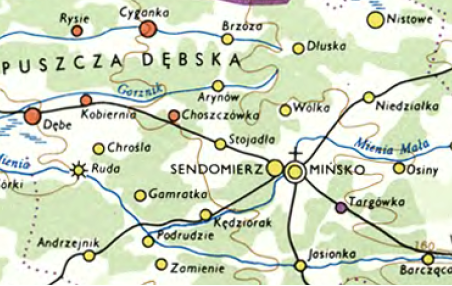
\includegraphics[width=1.0\linewidth]{
        Wólka Mińska - Mazowsze w drugiej połowie XVI wieku.png}
    \captionsetup{format=hang}
    \caption{Mapa miejscowości znajdujących się w~okolicy Mińska Mazowieckiego 
    w~połowie XVI~wieku opracowana w~1972~roku przez Instytut Historii 
    Polskiej Akademii Nauk \cite{palucki}.}
    \label{fig:wolka_minska_xvi}
\end{figure}

Jan Gomulski (ur.~1836~r. - zm.~1901~r.), najstarszy syn Piotra i~Marianny 
Gumulskich, 31~stycznia~1858~roku wziął ślub z~Agnieszką Piotrkowicz 
(ur.~1840~r. - zm.~1881~r.). Agnieszka Piotrkowicz urodziła się 
26~grudnia~1840~roku w~Budach Barcząckich, a jej rodzice pochodzili 
z~Dębego Wielkiego.

\newpage
\ifodd\value{page}\hbox{}\newpage\fi

% Przednia okładka podrozdziału
\includepdf{Mikanow_mapa_fin.png}

\section{Mikanów: 1882~r. - 1894~r.}

W~bieżącym


\newpage
\ifodd\value{page}\hbox{}\newpage\fi

% Przednia okładka podrozdziału
\includepdf{Karolina_mapa_fin.png}

\section{Karolina: 1896~r. - 2025~r.}

W~bieżącym
